\chapter{Dataset}

Object detection in minibars involves the use of computer vision techniques and object detection models to identify and track items inside the minibar. In this project, I trained photos that captured in minibar for getting better results in minibar.


\section{Processing Dataset}

\subsection{Objective}
Take pictures from minibar with webcam and label them for processing.Divide parts images for 80 percent train,
10 percent validation, 10 percent test.

\subsection{Libraries and Modules Used}
The process uses Python libraries and modules including pandas, numpy,os and some scripts. These libraries provide necessary functions for data processing.

\subsection{Scripts}
Scripts are mainly used for dividing pictures for train,test,validation; create labelmap txt for classes; create model, convert model tensorflow lite etc.

\subsection{Data Download and Processing}
Bounding boxes are created by label img. They are then filtered according to the classes specified by the user. 

In summary, user took images from minibar with different angles and all objects on the scene. Then labels all images with any label program for preparing training.

\subsection{Tensorflow Setup}
Tensorflow is required for using webcam or raspi cam with object recognition projects.For installing tensorflow we can follow this steps:

\subsection{Controlling version, then Installing Tensorflow and Python}
Start by setting up our Raspberry Pi with the latest version of Raspberry Pi OS with sudo apt update command.
Then install the required dependencies by running the sudo apt install libatlas-base-dev command.Then install python package with sudo apt install python3-pip and finally pip3 install tensorflow.

\subsection{Images From The Dataset}

\begin{figure}[!htbp]
    \centering
    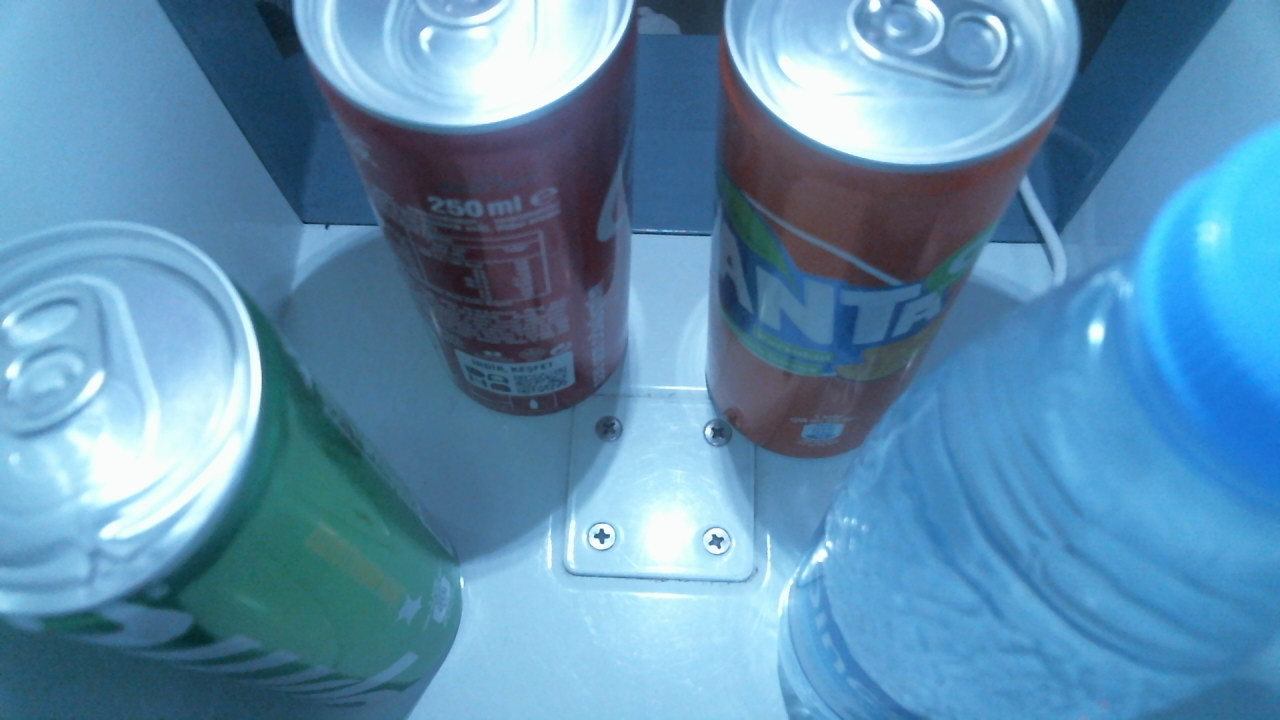
\includegraphics[width=1\textwidth]{Imgs/datasetphotos1.jpg}
    \caption{\label{fig:pic1}Photos from dataset.}
\end{figure}
\begin{figure}[!htbp]
    \centering
    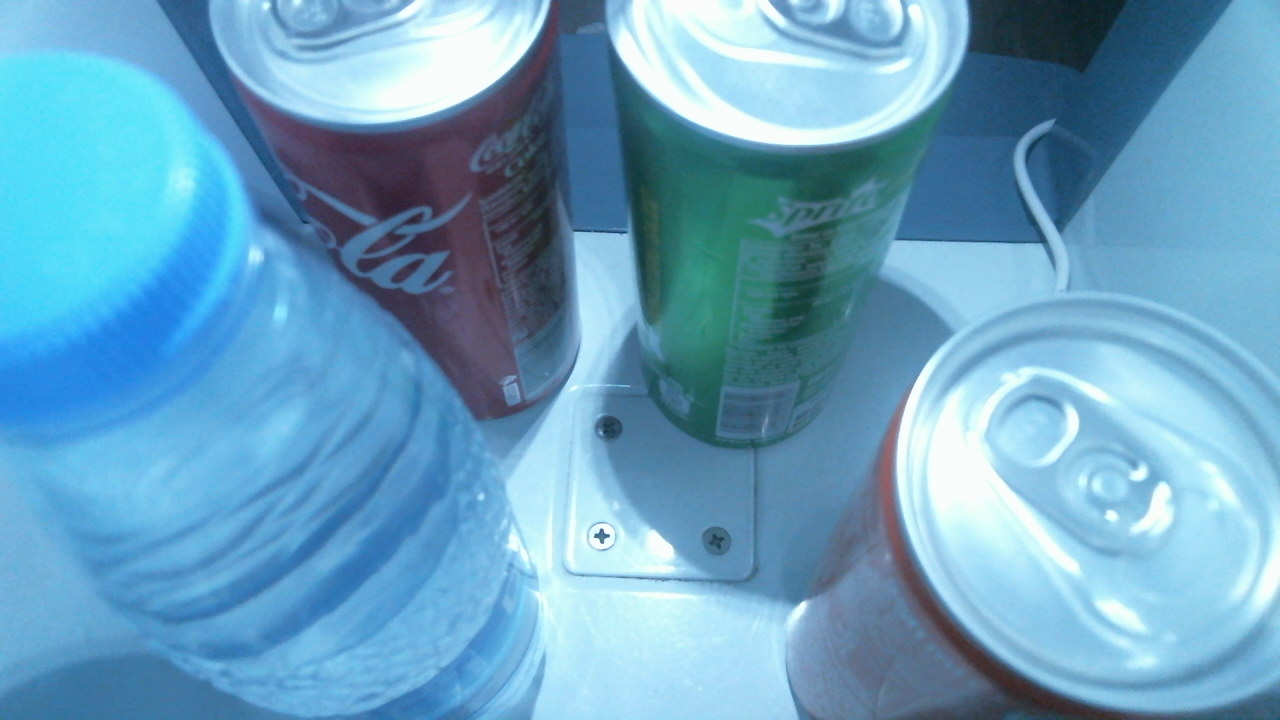
\includegraphics[width=1\textwidth]{Imgs/datasetphotos2.jpg}
    \caption{\label{fig:pic2}Photos from dataset.}
\end{figure}
\begin{figure}[!htbp]
    \centering
    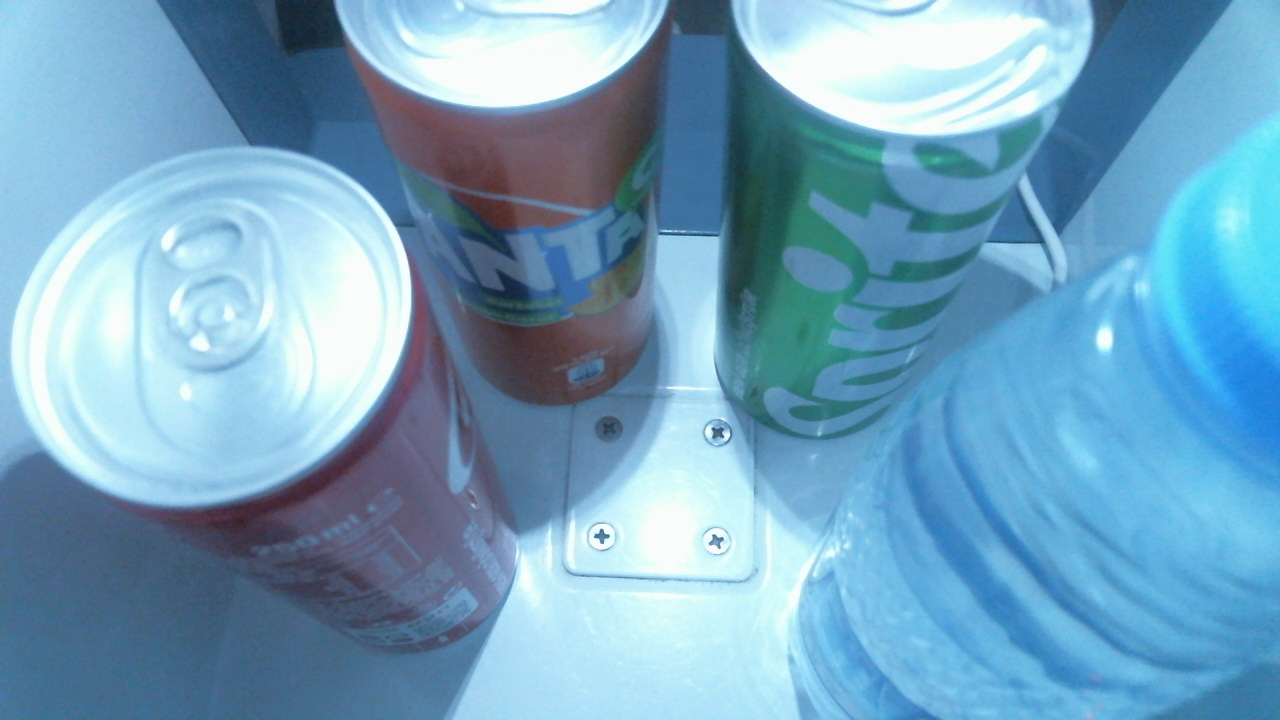
\includegraphics[width=1\textwidth]{Imgs/datasetphotos3.jpg}
    \caption{\label{fig:pic3}Photos from dataset.}
\end{figure}

\subsection{Resources}
Dataset can easily be created and labelled by How to Capture and Label Training Data to Improve Object Detection Model Accuracy namely youtube video.
